% =====================================================================
\chapter{The base scheme in detail}\label{ch:base}
% =====================================================================
Everything in this chapter is taken from Sections~III--V of~\cite{tan2023}. Equations are copied as printed; where the paper's wording matters we
quote it.

\section{System model}
\begin{figure}[H]
\centering
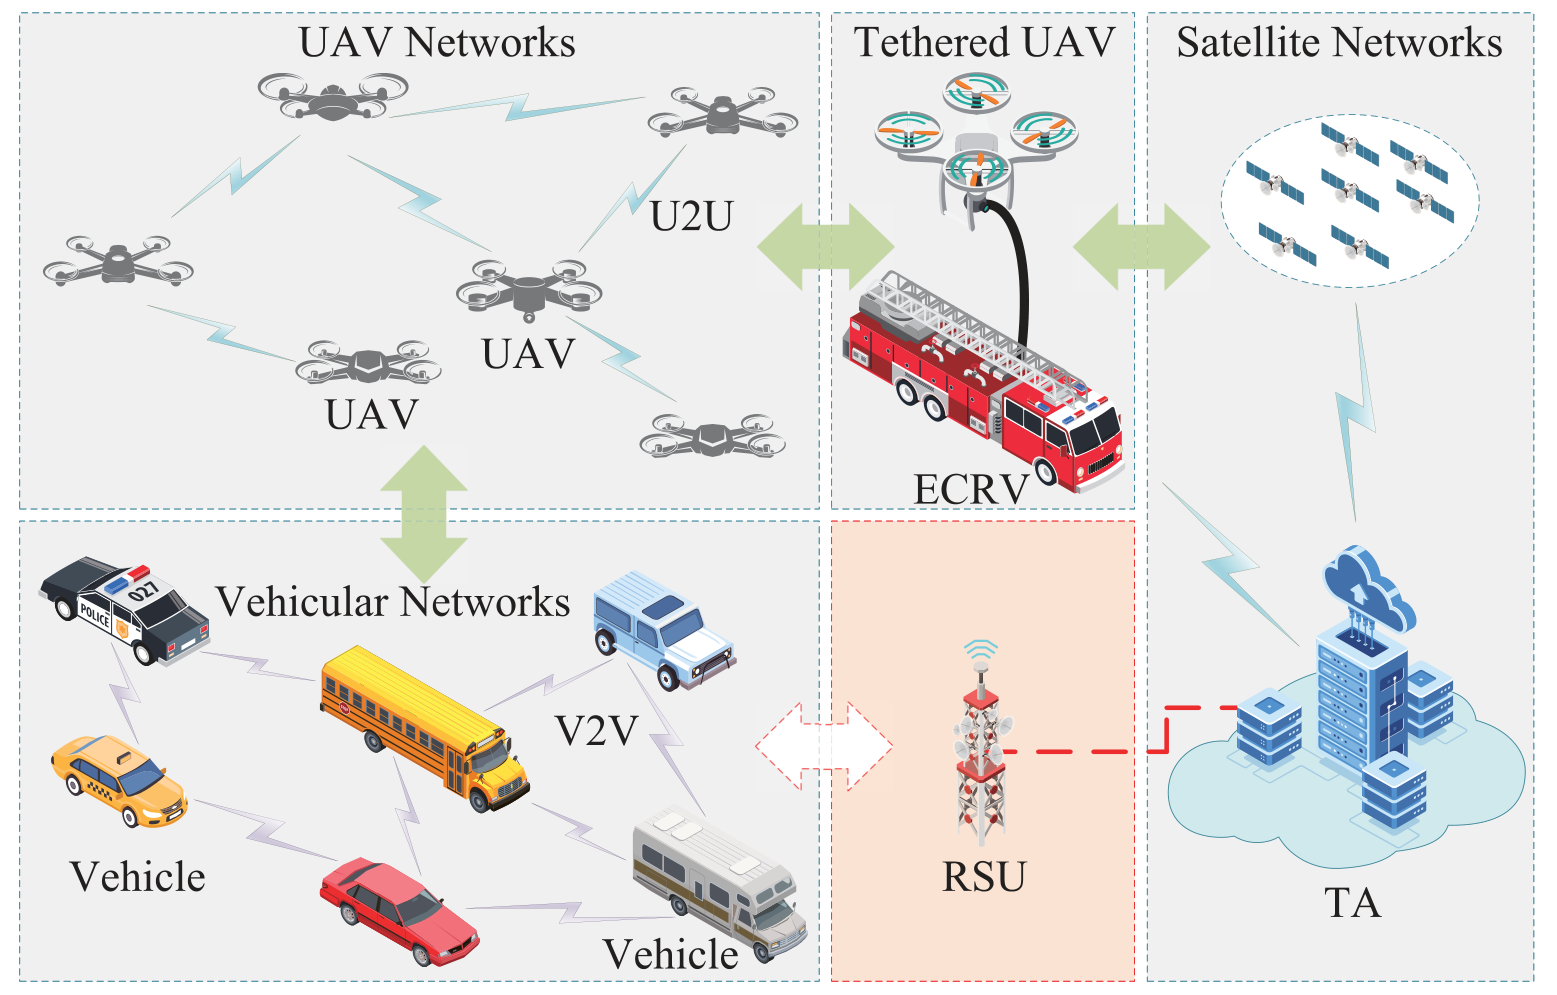
\includegraphics[width=0.78\linewidth]{paper_fig1_system_model.png}
\caption{System model of the TUAV-assisted infrastructure-less IoV, reproduced from Fig.~1 of the base paper~\cite{tan2023}. The UAV network (top left)
talks to the tethered UAV, which is powered through a cable by the ECRV. The ECRV reaches the trusted authority (TA) through the satellite network.
Vehicles (bottom left) communicate through the UAV network because the roadside unit (RSU) is out of service.}
\label{fig:sysmodel}
\end{figure}

\begin{claimbox}
``the data links between TA and TUAV are conducted with the secure communication channel, which takes the place of the dysfunctional edge RSUs.''
\quad ``the TUAVs utilize flexible tethered wires or cables as the power source instead of conventional batteries. The ECRV, as the auxiliary unit and
control center, maintains the wired power supply to the connected TUAV.'' \hfill (Section~III-D)
\end{claimbox}

\section{The protocol at a glance}
\begin{figure}[H]
\centering
\begin{tikzpicture}[font=\small,ph/.style={draw=black,fill=black!6,rounded corners=2pt,text width=11.4cm,align=left,inner sep=5pt},
  tg/.style={draw=black,fill=black!75,text=white,font=\small\bfseries,minimum width=1.9cm,minimum height=0.75cm}]
  \node[ph] (is) at (0,0) {\textbf{Initialisation} (TA, TUAV). The TA gives the TUAV $\langle id_{tu},s_{tu}\rangle$ and every UAV $\langle id_i,s_i\rangle$, and keeps a copy. The TUAV broadcasts $\langle \ts_{tu},\ID_{tu},R_{tu},Q_{tu}\rangle$.};
  \node[ph,below=0.45cm of is] (us) {\textbf{UAV signing} (each UAV). The UAV picks $r_i$, computes $\xi_i=h_1(r_i)$, $\ID_i$, $\upsilon_i$ and the credential $\Gamma_i$, and sends $\langle \ts_2,\ID_i,\xi_i,\upsilon_i,\Gamma_i\rangle$ to the TUAV.};
  \node[ph,below=0.45cm of us] (ga) {\textbf{Group authentication} (TUAV and TA, over the satellite). The TA uses $s_i$ to compute $\sigma_i,\psi_i,\mu_i,\delta_i$ (three pairings per UAV); the TUAV checks all UAVs with one product equation.};
  \node[ph,below=0.45cm of ga] (gd) {\textbf{Group key distribution} (TUAV to UAVs). The TUAV builds $\Lambda(x)=\kappa_{tu}\sum_i\omega_i\varphi_i+\prod_i(x-\sigma_i)$ and sends its coefficients; each UAV computes $\kappa_{tu}=\Lambda(\sigma_i)\bmod\sigma_i$.};
  \node[ph,below=0.45cm of gd] (du) {\textbf{Dynamic key updating} (TUAV). When UAVs join or leave, the TUAV builds a new $\Lambda^{*}(x)$ with a new key $\kappa^{*}_{tu}$; remaining members keep their $\sigma_i$.};
  \foreach \a/\b in {is/us,us/ga,ga/gd,gd/du}{\draw[-{Stealth[length=2.4mm]},thick] (\a.south) -- (\b.north);}
  \foreach \n/\t in {is/IS1--IS5,us/US1--US3,ga/GA1--GA4,gd/GD1--GD6,du/DU1--DU2}{\node[tg,left=0.25cm of \n] {\t};}
  \draw[-{Stealth[length=2.4mm]},thick,dashed] (du.east) -- ++(0.6,0) |- node[pos=0.25,right,font=\scriptsize,align=left]{on every\\ join or leave} (gd.east);
\end{tikzpicture}
\caption{The five phases of the base scheme, in order. The step labels on the left (IS, US, GA, GD, DU) are the ones used in Section~IV of the paper.
Solid arrows show the normal order; the dashed arrow shows that a key update repeats the key-distribution computation.}
\label{fig:phases}
\end{figure}

\begin{figure}[H]
\centering
\resizebox{\linewidth}{!}{%
\begin{tikzpicture}[font=\sffamily\small]
  \node[ent=uavc] (u) at (0,0) {UAV $\U_i$};
  \node[ent=hoc]  (t) at (6.6,0) {TUAV};
  \node[ent=deep] (a) at (13.2,0) {TA (via satellite)};
  \foreach \n in {u,t,a}{\draw[life] (\n.south) -- ++(0,-11.2);}
  \draw[msg=hoc] (6.6,-1.1) -- node[lbl,above]{IS5 \;$\langle \ts_{tu},\ID_{tu},R_{tu},Q_{tu}\rangle$ (broadcast)} (0,-1.1);
  \node[act=uavc,anchor=north] at (0,-1.4) {US1--US2: pick $r_i$; \;$\xi_i=h_1(r_i)$\\ $\ID_i=h_3(id_i,\ts_2,\xi_i)$, \;$\upsilon_i$, \;$\Gamma_i$};
  \draw[msg=uavc] (0,-3.0) -- node[lbl,above]{US3 \;$\langle\text{Request},\ts_2,\ID_i,\xi_i,\upsilon_i,\Gamma_i\rangle$} (6.6,-3.0);
  \draw[msg=deep,dashed] (6.6,-3.8) -- node[lbl,above]{GA1 \;upload $\langle\ts_2,\ID_i,\xi_i,\upsilon_i\rangle$ \;(satellite)} (13.2,-3.8);
  \node[act=deep,anchor=north] at (13.2,-4.1) {GA2: find $\langle id_i,s_i\rangle$; compute\\ $\sigma_i,\ \psi_i,\ \mu_i,\ \delta_i$\\ (3 pairings per UAV)};
  \draw[msg=deep,dashed] (13.2,-5.9) -- node[lbl,above]{GA2 \;$\langle\sigma_i,\psi_i,\mu_i,\delta_i\rangle$ \;(satellite)} (6.6,-5.9);
  \node[act=hoc,anchor=north] at (6.6,-6.2) {GA3--GA4: one product check\\ GD1--GD3: $\omega_i,\varphi_i,\kappa_{tu}$, \;$\Lambda(x)$, \;$S_i$};
  \draw[msg=hoc] (6.6,-8.0) -- node[lbl,above]{GD4 \;$\langle\text{ACK},\ts_3,\ID_i,S_i,\{a_k\}_{k=0}^{n}\rangle$ \;(to each UAV)} (0,-8.0);
  \node[act=uavc,anchor=north] at (0,-8.3) {GD5: check $S_i$\\ GD6: $\kappa_{tu}=\Lambda(\sigma_i)\bmod\sigma_i$};
  \node[draw=deep,fill=deep!6,rounded corners,font=\scriptsize\sffamily,text=deep,align=center] at (9.9,-10.3)
    {dashed arrows cross the satellite link; the coefficients $\{a_k\}$ travel in the clear};
\end{tikzpicture}}
\caption{Message flow of the base scheme between a UAV $\U_i$, the TUAV and the TA. Time runs from top to bottom. Solid arrows are local radio messages; dashed arrows cross the satellite link. Boxes show the local computation of each entity.}
\label{fig:baseflow}
\end{figure}

\section{Initialisation (IS)}
\begin{stepbox}{deep}{IS1--IS5 \;(Section IV-A)}
\steplabel{deep}{IS1.} TA $\to$ TUAV: $\langle id_{tu},s_{tu}\rangle$, ``safely shared only between TA and TUAV itself during the whole time''.\\
\steplabel{deep}{IS2.} TA $\to\U_i$: $\langle id_i,s_i\rangle$; ``both the TUAV and UAV identity sets are safely stored by TA''.\\
\steplabel{deep}{IS3.} Groups $\G_1,\G_2$ of prime order $q$, generator $P$, pairing $\hat e$, hashes $\BH,h_1,h_2,h_3,h_4$.\\
\steplabel{deep}{IS4.} The TUAV, ``with the effective range covering the entire region'', picks $r_{tu}$ and computes
\[ \ID_{tu}=h_2(id_{tu},r_{tu}),\qquad R_{tu}=r_{tu}\,h_2(\ts_{tu},s_{tu}),\qquad Q_{tu}=s_{tu}\,h_2(\ID_{tu},r_{tu})\,P. \]
\steplabel{deep}{IS5.} The TUAV broadcasts $\langle\ts_{tu},\ID_{tu},R_{tu},Q_{tu}\rangle$ periodically.
\end{stepbox}

\section{UAV signing (US) and group authentication (GA)}
\begin{stepbox}{uavc}{US1--US3 \;(Section IV-B1, each UAV)}
\steplabel{uavc}{US1.} Pick random $r_i$; \;$\xi_i=h_1(r_i)$; \;$\ID_i=h_3(id_i,\ts_2,\xi_i)$.\\
\steplabel{uavc}{US2.} $\upsilon_i=h_4(\ID_i,\ID_{tu},\ts_2,\xi_i)$ and
\begin{equation}\label{eq:gamma}
\Gamma_i=\big[s_i\,h_3(\ID_i,\ts_2,s_i)\,R_{tu}-h_1(s_i\xi_i)\big]P-\upsilon_i\,h_1(r_i)\,Q_{tu}.
\end{equation}
\steplabel{uavc}{US3.} Send $\langle\text{Request},\ts_2,\ID_i,\xi_i,\upsilon_i,\Gamma_i\rangle$ to the TUAV.
\end{stepbox}

\begin{stepbox}{hoc}{GA1--GA4 \;(Section IV-B2, TUAV and TA)}
\steplabel{hoc}{GA1.} TUAV checks $\ts_2$ and $\upsilon_i$ and ``uploads'' $\langle\ts_2,\ID_i,\xi_i,\upsilon_i\rangle$ ``to the remote TA''.\\
\steplabel{hoc}{GA2.} TA recovers $\langle id_i,s_i\rangle$ for $\ID_i$ and computes, for every $i$,
\begin{gather*}
\sigma_i=h_1(s_i\xi_i)P,\qquad \psi_i=\hat e(\Gamma_i+h_1(s_i\xi_i)P,\,P),\\
\mu_i=\hat e(h_3(\ID_i,\ts_2,s_i)P,\,s_iP),\qquad \delta_i=\hat e(s_{tu}P,\,\upsilon_i\xi_iP),
\end{gather*}
and forwards $\langle\sigma_i,\psi_i,\mu_i,\delta_i\rangle_{i\in[1,n]}$ to the TUAV.\\
\steplabel{hoc}{GA3.} TUAV checks
\begin{equation}\label{eq:ga3}
\prod_{i=1}^n\psi_i\Big(\prod_{i=1}^n\delta_i\Big)^{h_2(\ID_{tu},r_{tu})}\overset{?}{=}\prod_{i=1}^n\mu_i^{R_{tu}} .
\end{equation}
\steplabel{hoc}{GA4.} ``If matches, the validity of the vehicles can be proved.''
\end{stepbox}

\begin{lemma}[Correctness of GA3, the paper's Eq.~(1)]\label{lem:ga3}
For honestly generated requests, Eq.~\eqref{eq:ga3} holds.
\end{lemma}
\begin{proof}
Write $h_2=h_2(\ID_{tu},r_{tu})$ and $h_3=h_3(\ID_i,\ts_2,s_i)$. By \eqref{eq:gamma} and $h_1(r_i)=\xi_i$,
$\Gamma_i+h_1(s_i\xi_i)P=s_ih_3R_{tu}P-\upsilon_i\xi_iQ_{tu}$, so by bilinearity
$\psi_i=\hat e(s_ih_3R_{tu}P,P)\cdot\hat e(\upsilon_i\xi_iQ_{tu},P)^{-1}$. Since $Q_{tu}=s_{tu}h_2P$,
$\delta_i^{h_2}=\hat e(s_{tu}h_2P,\upsilon_i\xi_iP)=\hat e(\upsilon_i\xi_iQ_{tu},P)$. The two factors cancel and
$\psi_i\delta_i^{h_2}=\hat e(h_3P,s_iP)^{R_{tu}}=\mu_i^{R_{tu}}$. Multiply over $i$.
\end{proof}

\section{Group key distribution (GD) and dynamic update (DU)}
\begin{stepbox}{hoc}{GD1--GD6 \;(Section IV-C)}
\steplabel{hoc}{GD1.} TUAV takes the decrypting keys $\sigma_i=h_1(s_i\xi_i)P$, builds $\omega_i=\prod_{j\neq i}\sigma_j$ and $\varphi_i\equiv\omega_i^{-1}\bmod\sigma_i$,
and selects the group key $\kappa_{tu}\in\Zq$.\\
\steplabel{hoc}{GD2.} TUAV constructs
\begin{equation}\label{eq:lambda}
\Lambda(x)=\kappa_{tu}\sum_{i=1}^n\omega_i\varphi_i+\prod_{i=1}^n(x-\sigma_i)=\sum_{k=0}^{n}a_kx^k .
\end{equation}
\steplabel{hoc}{GD3.} $S_i=\BH(\ts_3,\ID_i,\,s_{tu}h_2(\ID_{tu},r_{tu})\,\sigma_i)$; the acknowledgement ``is delivered one by one to each vehicle''.\\
\steplabel{hoc}{GD4.} Packet $\langle\text{ACK},\ts_3,\ID_i,S_i,\{a_k\}_{k\in[0,n]}\rangle$.\\
\steplabel{uavc}{GD5.} UAV checks $S_i\overset{?}{=}\BH(\ts_3,\ID_i,h_1(s_i\xi_i)Q_{tu})$.\\
\steplabel{uavc}{GD6.} UAV rebuilds $\Lambda(x)$ from $\{a_k\}$ and computes $\kappa_{tu}=\Lambda(\sigma_i)\bmod\sigma_i$.
\end{stepbox}
\begin{stepbox}{hoc}{DU1--DU2 \;(Section IV-D)}
\steplabel{hoc}{DU1.} For $\ominus$ removed and $\oplus$ joining UAVs, the TUAV picks $\kappa^*_{tu}$ and computes
$\Lambda^*(x)=\prod_{i=1}^{n-\ominus+\oplus}(x-\sigma_i)+\kappa^*_{tu}\big(\sum_{i=1}^{n-\ominus+\oplus}\omega_i\varphi_i\big)$.\\
\steplabel{uavc}{DU2.} ``all the legitimate UAVs could easily extract $\kappa^*_{tu}$ with $\kappa_{tu}=\Lambda^*(\sigma_i)\bmod\sigma_i$'' -- using the
\emph{same} $\sigma_i$ as before.
\end{stepbox}

\begin{lemma}[Correctness of GD6 by the CRT]\label{lem:gd6}
If the $\sigma_i$ are pairwise coprime and $\kappa_{tu}<\sigma_i$ for all $i$, then $\Lambda(\sigma_i)\bmod\sigma_i=\kappa_{tu}$ for every member $i$.
\end{lemma}
\begin{proof}
At $x=\sigma_i$ the product in \eqref{eq:lambda} contains the factor $(\sigma_i-\sigma_i)=0$, so $\Lambda(\sigma_i)=\kappa_{tu}\sum_j\omega_j\varphi_j$.
For $j\neq i$, $\omega_j$ contains the factor $\sigma_i$, so $\omega_j\varphi_j\equiv0\pmod{\sigma_i}$; and $\omega_i\varphi_i\equiv1\pmod{\sigma_i}$ by
the choice of $\varphi_i$ (Theorem~\ref{thm:crt}). Hence $\Lambda(\sigma_i)\equiv\kappa_{tu}\pmod{\sigma_i}$, and as $\kappa_{tu}<\sigma_i$ the remainder
is $\kappa_{tu}$ itself.
\end{proof}

\begin{remark}[Point or integer?]\label{rem:typing}
The paper writes $\sigma_i=h_1(s_i\xi_i)P$, a curve point, yet uses it as a CRT modulus and as a root of a polynomial over the integers. Any
implementation must therefore map $\sigma_i$ to an integer (for instance a fixed integer encoding of the point, or a prime derived from the same hash),
and the coefficients $a_k$ must be kept as integers -- otherwise ``$\bmod\ \sigma_i$'' in GD6 is undefined. All our results hold for \emph{every} such
integer reading; nothing depends on which encoding is chosen.
\end{remark}

\section{What the paper claims}
\begin{claimbox}
\textbf{Section IV-D:} ``the group key updating mechanism supports multi-device revocation and new device participation \dots\ the dynamic key batch
updating process can be securely executed in the open wireless environment since the malicious entities that successfully collect the coefficient set
$\{a_i\}_{i\in[0,n]}$ can not acquire the $\kappa_{tu}$ without the correct decrypting key $\sigma_i$.''\\[3pt]
\textbf{Proof of Theorem 4:} ``The certificateless authentication is adopted, where the partial secret set $\langle s_i,s_{tu}\rangle$ of TUAV and UAVs is
generated and determined by TA. On the other hand, the UAV itself also randomly generates $r_i$ as the partial key \dots''\\[3pt]
\textbf{Proof of Theorem 5:} ``The remaining legitimate UAVs could always use the previously issued key to decrypt the new $\kappa_{tu}$ with the updated
$\Lambda(x)$, if the $\sigma_i$ has not been removed by TUAV.''\\[3pt]
\textbf{Table II:} the proposed scheme is ticked (\yes) for all of F1--F11: unforgeability, conditional privacy, session key establishment,
\textbf{key escrow resilience}, scalability, dynamic identity updating, \textbf{forward secrecy}, batch validation, unlinkability,
\textbf{non-repudiation} and replay attack resilience.
\end{claimbox}

\begin{center}
\small
\begin{tabularx}{\linewidth}{@{}X c X@{}}
\toprule
\textbf{Claim in~\cite{tan2023}} & \textbf{Paper} & \textbf{This report}\\
\midrule
Key escrow resilience (Table II, F4) & \yes & \no\ fails: the TA can sign for any UAV (F1, Theorem~\ref{thm:taforge})\\
Non-repudiation (Table II, F10) & \yes & \no\ fails: the TA could have produced any request (F1)\\
``supports multi-device revocation'' (IV-D, Thm.~5) & \yes & \no\ fails: a removed UAV computes the new key (F2a)\\
New-device participation is secure (IV-D) & \yes & \no\ fails: a newcomer reads old keys (F2b)\\
Coefficients reveal nothing without a $\sigma_i$ (IV-D) & \yes & \no\ fails: a passive outsider gets all keys (F2c)\\
Forward secrecy (Table II, F7) & \yes & \no\ fails: a leaked $s_i$ opens all past keys (F3)\\
\bottomrule
\end{tabularx}
\end{center}
